\begin{exercice*}
    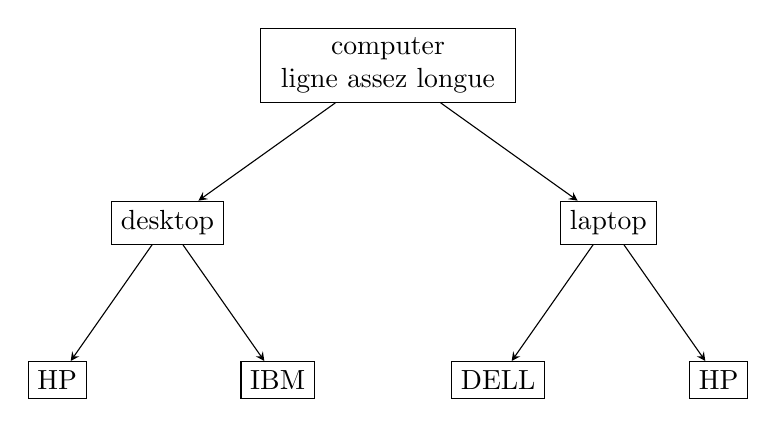
\begin{tikzpicture}[>=stealth,yscale=2,xscale=1.4]  
        % xscale et yscale permettent d'ajuster largeur et hauteur
        
        % positionner les nœuds
        \node(comp) at (4,3)[rectangle,draw,text width=3cm,text centered] {computer\\ligne assez longue};
        \node(desk) at (2,2)[rectangle,draw] {desktop};
        \node(lap)  at (6,2)[rectangle,draw] {laptop}; 
        \node(HPl)  at (1,1)[rectangle,draw] {HP};     
        \node(IBM)  at (3,1)[rectangle,draw] {IBM};    
        \node(DELL) at (5,1)[rectangle,draw] {DELL};   
        \node(HPr)  at (7,1)[rectangle,draw] {HP};        
                              
        % tirer les liens
        \draw[->] (comp) -- (desk); 
        \draw[->] (comp) -- (lap);
        \draw[->] (desk) -- (HPl); 
        \draw[->] (desk) -- (IBM); 
        \draw[->] (lap)  -- (DELL); 
        \draw[->] (lap)  -- (HPr); 
    \end{tikzpicture}
\end{exercice*}
\begin{corrige}
    %\setcounter{partie}{0} % Pour s'assurer que le compteur de \partie est à zéro dans les corrigés
    %\phantom{rrr}    
    \dots
\end{corrige}

